\section{Methods}
\label{sec:methods}
In this section, we briefly describe the approach by Godard \etal~\cite{Godard_2017_CVPR}.
We then explain atrous convolutions and how we extended Godard \etal's architecture with atrous convolutions.

\subsection{Monocular Depth Estimation}
\label{sec:methods:depth-estimation}
Monocular depth estimation can be treated as a stereo reconstruction problem, where a left an right image ($I^l$ and $I^r$) are available during training.
The left image is fed through an encoder-decoder CNN, which outputs a disparity map w.r.t. the right image ($d^r$).
\begin{figure}
    \centering
    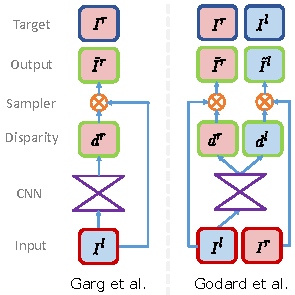
\includegraphics[width=0.8\linewidth]{images/architecture/monodepth.pdf}
    \caption{Monocular depth estimation via stereo reconstruction: naive approach by Garg et al.~\cite{garg2016unsupervised} and method with left-right consistency (figure adapted from Godard et al.~\cite{Godard_2017_CVPR}).}
    \label{fig:monodepth}
\end{figure}
This disparity map is applied to the left image using backward warping with bilinear interpolation in order to obtain the reconstructed right image $\Tilde{I}^r$ (see \figurename~\ref{fig:monodepth}, left column).
The CNN can be trained with an appearance-based loss function that measures the photometric difference between $I^r$ and $\Tilde{I}^r$.

Godard \etal's~\cite{Godard_2017_CVPR} main contribution is the idea of left-right consistency: instead generating only the right disparity map, the CNN outputs a pair of corresponding left and right disparity maps ($d^l$ and $d^r$).
The left image is further warped with the right disparity map and vice versa (see \figurename~\ref{fig:monodepth}, right column).
The loss function consists of three weighted terms:
\begin{align}
    C_s = \alpha_{ap}C_{ap} + \alpha_{ds}C_{ds} + \alpha_{lr}C_{lr} \quad .
\end{align}
$C_{ap}$ is the appearance-based loss, $C_{ds}$ is a disparity smoothness term, which penalizes high derivatives in the disparity maps, and $C_{lr}$ is a left-right consistency penalty, which ensures that the left and right disparity maps agree.
Each term is weighted with an $\alpha$ value respectively.
Additionally, this loss is computed and summed across four different output scales: $C = \sum_{s=1}^4 C_s$.

We use these basic ideas (image reconstruction, smoothness, left-right consistency), but instead of a standard ResNet50 backbone, we experiment with atrous convolutions.


\subsection{Atrous Convolutions}
The output $g(i)$ at index  $i$ of a 1D atrous convolution $w$ is given by
\begin{align}
    g(i) = \sum_{k=1}^K x(i + rk) w(k) \quad ,
\end{align}
where $x$ is the input and $K$ is the filter size. The filter dilation $r$ specifies the rate at which the input is sampled. A standard convolution is a special case of an atrous convolution, where $r = 1$. 
The notion of an atrous convolution can be generalized to 2D for vision problems straightforward. \figurename~\ref{fig:atrous-convolution} shows a 2D atrous convolution with $r=2$.

We employ the idea of an Atrous Spatial Pyramid Pooling (ASPP) block~\cite{chen2018deeplab}, which contains several atrous convolutions with different atrous rates in parallel (see \figurename~\ref{fig:aspp}).
This is motivated by classical image pyramid methods~\cite{Witkin1987,quam1987hierarchical}, which process images at different spatial scales. 
Since varying atrous rates results in filters of different spatial dimensions, an ASPP block resembles a feature map at different spatial scales.
The atrous convolutions, along with a global averaging pooling layer, are concatenated and passed through a $1 \times 1$ convolution, which reduces the number of channels to 256.

\subsection{Output Stride}
\begin{figure}
    \centering
    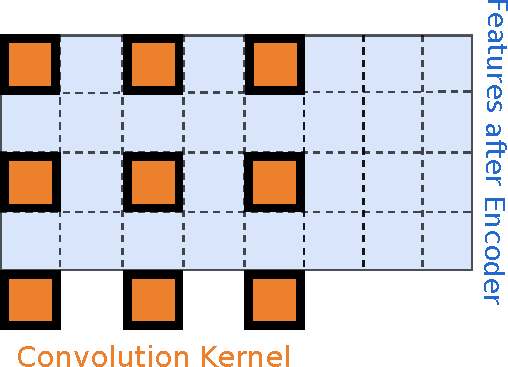
\includegraphics[width=0.6\linewidth]{images/architecture/os64-atrous-conv-with-text.pdf}
    \caption{A $4 \times 8$ feature map processed with an atrous convolution with rate 2.
    Some of the filter weights are out of the image range, which results in boundary issues.
    This effect is even stronger for convolutions with larger atrous rates.}
    \label{fig:output-stride}
\end{figure}
The output stride of a feature map is the factor by which its spatial dimensions are smaller than those of the input image.
Each ResNet block changes the output stride by a factor determined by the stride of its main convolutional layer.
In a standard ResNet50, each ResNet block has a stride of 2, which yields an output stride of 64 after the encoder.
This was also used in the monocular depth estimation architecture by Godard \etal, resulting in a $4\times8$ feature map after the encoder for $256 \times 512$ input images.
But in order to obtain feature responses at different spatial scales using atrous convolutions (with varying kernel size and thus FOVs), a certain size of image is required as illustrated in \figurename~\ref{fig:output-stride}.
Hence, we made the output stride in our network architecture variable by adapting the ResNet block output strieds.

\subsection{Our Architecture}
\begin{figure*}
\begin{center}
    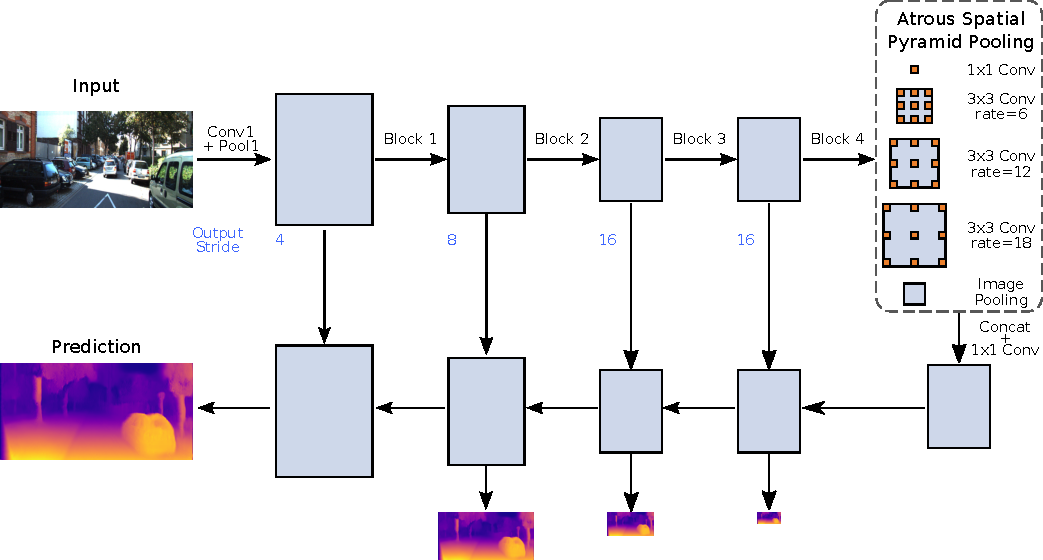
\includegraphics[width=0.9\linewidth]{images/architecture/architecture.pdf}
\end{center}
    \caption{Overview of our architecture.
    The input image is fed through a ResNet50 architecture, consisting of four blocks.
    Final feature maps of ResNet50 are passed to the ASPP block, which processes its input at several spatial scales in parallel.
    The decoder then upsamples the image again, while taking low-level features from the skip-connections and outputting disparity maps at multiple spatial scales.}
    \label{fig:our_architecture}
\label{fig:short}
\end{figure*}
\figurename~\ref{fig:our_architecture} shows a sketch of our architecture.
We use the same basic setup as Godard \etal~\cite{Godard_2017_CVPR}, i.e. a ResNet50 backbone, skip connections between the encoder and the decoder and output disparities at multiple spatial scales.
Our main contribution is the extension of the encoder by an ASPP block, inspired by the DeepLab architecture~\cite{chen2018deeplab}. For our main experiments, we insert the ASPP module after the final layer of the ResNet50, since this placement has proven to work well in other work~\cite{chen2018encoder, Fu2018}. Alternative choices, e.g. in between ResNet blocks, are also possible (see Section \ref{section:experiments:atrous-encoder} and supplement \ref{appendix:atrous-encoder}).

The ASPP block introduces additional parameters to the architecture.
By processing the ASPP block output with a $1\times 1$ convolution, we reduce the number of feature maps to 256 after the encoder, compared to 2048 feature maps in the original architecture.
Since this reduces the decoder input dimensionality, we effectively keep the number of parameters identical to the original architecture at 58.4 million\footnote{While inspecting the TensorFlow implementation by Godard \etal, we found that their ResNet50-based architecture, in fact, had 58.4 million parameters, instead of the specified 48 million.}.



